\section{Security Evaluation}\label{sec:Security_Evaluation}
\begin{questions}
\question{} What is the purpose with a security review and when should it be performed?
  \begin{solution}
    A security review is intended to perform a general ``sanity'' check that the chosen Security Architecture makes sense.
    It also helps identify potential gaps in the Security Architecture that might have been missed.
    It can also provide a business evaluation of the chosen architecture to find business consequences.
    Lastly, we take the perspective of an attacker attempting to break into the system.

    Generally, this is done after the Architecture and Design is completed, but performing it regularly during these steps also works.
  \end{solution}

\question{} At which four main levels do you typically perform a security evaluation?
  \begin{solution}
    \begin{enumerate}[noitemsep]
    \item Security Architecture Review
    \item Design against Requirements Review
    \item Design Review
    \item Implementation Review
    \end{enumerate}
  \end{solution}

  \begin{parts}
  \part{} At which occasion should they be done?
    \begin{solution}
      \begin{enumerate}[noitemsep]
      \item After the Security Architecture design selections.
      \item Before the Security Design Specification.
      \item After the Security Design Specification.
      \item Before the system's release.
      \end{enumerate}
    \end{solution}
  \end{parts}

\question{} Mention three different aspects to consider at an architecture ``sanity check'' review.
  \begin{solution}
    \begin{enumerate}[noitemsep]
    \item System purpose vs. Security
    \item Usability Check
    \item Administrative Burden
    \end{enumerate}
  \end{solution}

  \begin{parts}
  \part{} For each aspect, list what should be considered?
    \begin{solution}
      \begin{enumerate}[noitemsep]
      \item
        \begin{itemize}[noitemsep]
        \item Does the chosen Security Architecture change any system functions?
        \item Are the security functions adding any new system properties?
        \item Can these new security functions be accepted the end-users?
        \end{itemize}
      \item
        \begin{itemize}[noitemsep]
        \item Will the security functions have any direct usability considerations?
        \item If they do, are they acceptable?
        \item Is it possible to modify the system to make it easier to use while maintaining security?
        \end{itemize}
      \item
        \begin{itemize}[noitemsep]
        \item Which routines and security policies are necessary to make the architecture functional?
        \item How costly is it to maintain the routines and policies?
        \item How much will the system be dependent on manual routines?
        \end{itemize}
      \end{enumerate}
    \end{solution}
  \end{parts}

\question{} Mention three different aspects to consider at an architecture business review.
  \begin{solution}
    \begin{enumerate}[noitemsep]
    \item Security Control
    \item Customer Relations
    \item Business Risks and Opportunities
    \end{enumerate}
  \end{solution}

  \begin{parts}
  \part{} For each aspect, list what should be considered?
    \begin{solution}
      \begin{enumerate}[noitemsep]
      \item
        \begin{itemize}[noitemsep]
        \item Who is in control of the system's security funcctions?
        \item Will the security control give the party controlling these an advantage?
        \item If so, make sure the security controls are kept within the business' domains.
        \end{itemize}
      \item
        \begin{itemize}[noitemsep]
        \item Will the suggested Security Architecture influence any existing or future customer relations?
        \item If so, this \emph{\textbf{MUST}} be highlighted and discussed with the client.
        \end{itemize}
      \item
        \begin{itemize}[noitemsep]
        \item Will the architecture influence the current business in a direct or indirect way?
        \item If so, can we make sure the business implications are favorable?
        \end{itemize}
      \end{enumerate}
    \end{solution}
  \end{parts}

\question{} What do you perform during a security requirements review?
  \begin{solution}
    The Security Requirements are revisted to ensure the current System Architecture addresses \textbf{ALL} the mandator requirements.
    Any that are missing are added and the Security Design is updated to reflect this.
  \end{solution}

\question{} Mention four different aspects to consider at a design review.
  \begin{solution}
    \begin{enumerate}[noitemsep]
    \item Standards Review
    \item Data Representation
    \item Protocols
    \item Review of New Designs
    \end{enumerate}
  \end{solution}

  \begin{parts}
  \part{} For each aspect, list what should be considered?
    \begin{solution}
      \begin{enumerate}[noitemsep]
      \item
        \begin{itemize}[noitemsep]
        \item Are standards used when possible?
        \item Are the chosen standards appropriate for this use-case?
        \item Are our own design choices compliant with the relevant standards?
        \end{itemize}
      \item
        \begin{itemize}[noitemsep]
        \item Is the data format used appropriate for the system's functions?
        \item Is the data representation in a protected format when needed?
        \item Is the data accessible whenever it is needed?
        \item Is the footprint required for securing this data acceptable?
        \end{itemize}
      \item
        \begin{itemize}[noitemsep]
        \item Are all new protocol designs evaluated and verified?
        \item Are the protocol's performance figures acceptable?
        \end{itemize}
      \item
        \begin{itemize}[noitemsep]
        \item In the new designs, do the parts have security soundness?
        \item Is ti possible to verify (theoretically or formally) any new design choices?
        \item Is the performance of these new design choices acceptable?
        \item Has the new design been reviewed by independent experts?
        \end{itemize}
      \end{enumerate}
    \end{solution}
  \end{parts}

\question{} Describe a process for issuing and security testing of a software product.
  \begin{solution}
    The software product goes from the owner to the requirements board with the desired result.
    The requirements board uses these to generate the software's requirements, which is handed off to the engineers.
    From there, it is designed, implemented, tested, delivered, reviewed, redesigned, etc.\ until it meets the client's criteria.
    From there, it moves onto penetration testing, to ensure that it works.
    Once the software is validated through penetration testing, it is given to the client as a release candidate.
  \end{solution}

  \begin{parts}
  \part{} What is the role in the process for the security officer, the security architect, the security master and security penetration tester respectively?
    \begin{solution}
      \begin{itemize}[noitemsep]
      \item The Security Officer is the one that generates the first round of security requirements for the product.
      \item The Security Architect is the one who finds potential vulnerabilities, creates an architecture for them, and ensures that they are handled.
      \item The Security Master ensures that the security protocols addressed in the Security Requirements are met during developement.
      \item The Penetration Testers attempt to break into the program by attacking and stealing information that should not be stolen from the program, to determine additional vulnerabilities or items that were missed.
      \end{itemize}
    \end{solution}
  \end{parts}

\question{} Give examples of things to consider during a performance review of a design?
  \begin{solution}
    \begin{itemize}[noitemsep]
    \item Execution speed of the design and the algorithms chosen.
    \item The memory usage of the chosen algorithms and their required parameters and keys.
    \item Is there a need for special hardware?
      \begin{itemize}[noitemsep]
      \item If so, what is the execution speed/memory usage of this hardware?
      \end{itemize}
    \item Does any part of this Security Design have real-time performance impacts?
    \item Are there any performance bottlenecks in the design?
    \end{itemize}
  \end{solution}

\question{} What is the purpose of trying to ``measure'' the security of a design?
  \begin{solution}
    To put a quantifiable metric on a solution.
    By using numbers, we know what we need to design for, which design is the most effective, what changes must be made, etc.
    We can also track improvements to the system, among other statistics that could be made.
  \end{solution}

\question{} A simple security measurement takes three basic security characteristics into account:
  \begin{parts}
  \part{} Which three characteristics are then measured and how do you combine the measurements to get an overall measurement of a system?
    \begin{solution}
      \begin{enumerate}[noitemsep]
      \item Confidentiality
      \item Integrity
      \item Availability
      \end{enumerate}

      Each of these is given a score according to a function that is determined from the weighting of the items in that portion of the evaluation tree.
      These are combined according to another weighted function to produce a final result.

      \begin{equation}\label{eq:CIA_Functions}
        \begin{aligned}
          \langle f_{1}(\text{Confidentiality}), &f_{2}(\text{Integrity}), f_{3}(\text{Availability}) \rangle \\
          g(f_{1}, f_{2}, f_{3}) &= w_{1} f_{1} + w_{2}f_{2} + w_{3}f_{3} \\
        \end{aligned}
      \end{equation}
    \end{solution}
  \end{parts}

\question{} Consider the smart card security system in \Cref{fig:Smart_Card_Security_System}.
  Assume the side-channel and physical channel break are equal important and the overall smart card security is the minmum strength of the two nodes.
  Calculate the smart card security score using the weighted weakest link approach.
  \begin{figure}[h!]
    \centering
    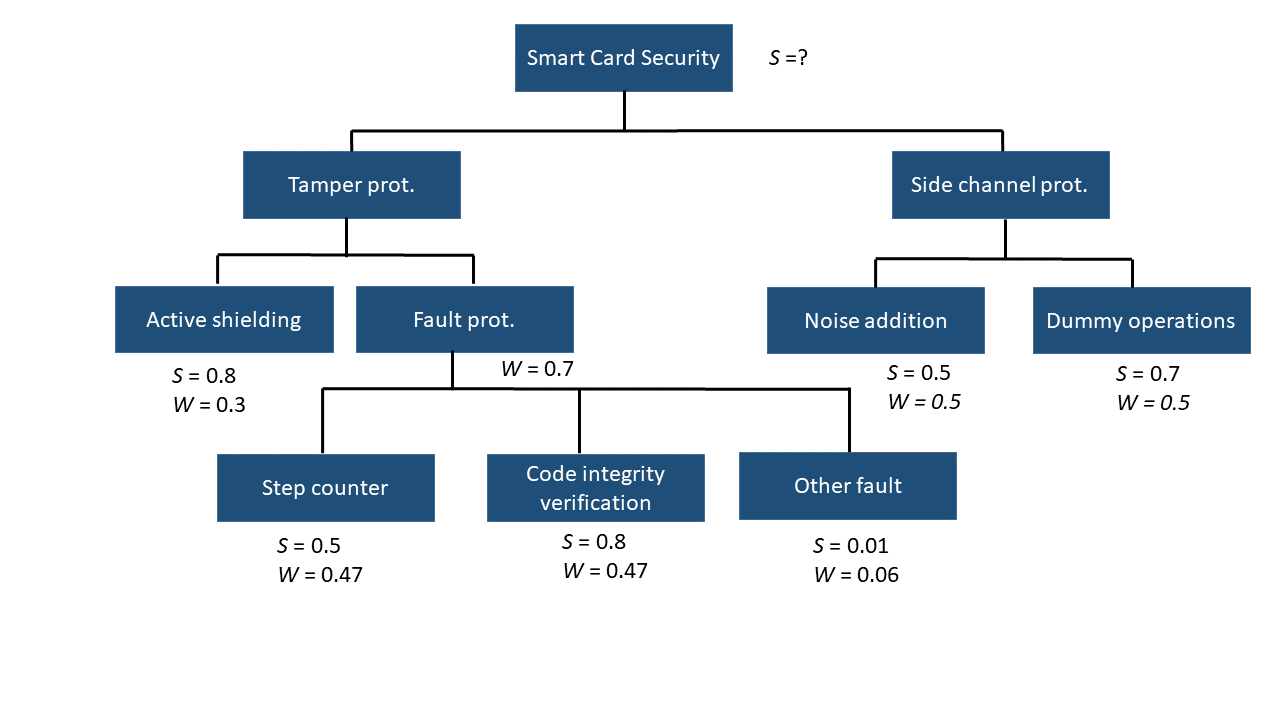
\includegraphics[scale=0.35]{./Drawings/EITP20-Secure_Systems_Engineering/Smart_Card_Security_System.png}
    \caption{Smart Card Security System}
    \label{fig:Smart_Card_Security_System}
  \end{figure}
  \begin{solution}
    \begin{equation}\label{eq:Weighted_Weakest_Link}
      \begin{aligned}
        WWL &= \sqrt{WS \times WW} \\
        WS &= \sum\limits_{k=1}^{n} S_{k}W_{k} \\
        WW &= \min \left( \frac{S_{1}}{NW_{1}}, \frac{S_{2}}{NW_{2}}, \ldots, \frac{S_{n}}{NW_{n}} \right) \\
        NW_{k} &= \frac{W_{k}}{\max{W_{1}, W_{2}, \ldots, W_{n}}} \\
        W_{\mathrm{Total}} &= \sum\limits_{k=1}^{n} W_{k} = 1
      \end{aligned}
    \end{equation}
  \end{solution}

\question{} How can the sensitivity for a certain security component be calculated?
  \begin{solution}
    \begin{equation}\label{eq:Sensitivity_Index}
      SI_{\text{Component}} = \frac{\partial S(\text{Root})}{\partial S(\text{Component})}
    \end{equation}
  \end{solution}

\question{} What is a CVE database? Which organizations maintain global CVEs?
  \begin{solution}
    \begin{description}[noitemsep]
    \item[C] Common
    \item[V] Vulnerabilities
    \item[E] Exposures
    \end{description}
    A CVE is a database of software vulnerabilities and exposure problems that have been recorded and written in a standard language to ensure the software is secured properly.

    NIST maintains a CVE, and MITRE does too.
  \end{solution}

\question{} What are the three basic categories for which CVE scoring is based
  \begin{solution}
    CVEs are usually scored using the CVSS Scoring Principle.
    \begin{enumerate}[noitemsep]
    \item Basic Metric Group
    \item Temporal Metric Group
    \item Environmental Metric Group
    \end{enumerate}
  \end{solution}

  \begin{parts}
  \part{} Briefly explain each of the three categories and which security aspects are considered for each of them?
    \begin{solution}
      \begin{enumerate}[noitemsep]
      \item These are items that are constant over any amount of time and across any user environment.
        Typically, they are the ways to exploit a vulnerability or exposure or the effects of the vulnerability or exposure.
      \item These are vulnerabilities that may change over time.
        These are typically going to change over time as the ability to exploit this documented code is patched and reviewed.
      \item These vulnerabilities are dependent on the particular user's environment.
        These are unique to every case and cannot be used everywhere.
      \end{enumerate}
    \end{solution}
  \end{parts}

\question{} A communication product have three different categories of weaknesses, buffer overflow, TPM weaknesses, and authentication weakness with the CVE list below. Calculate an overall vulnerability score for the product (use the NIST CVE database to obtain the individual scores).
  \begin{parts}
  \part{} Buffer overflow: CVE--2019--2304, CVE--2019--2242, CVE--2019--10572
  \part{} TPM:\@ CVE--2019--16863, CVE--2018--6622
  \part{} Authentication: CVE--2019--3768, CVE--2019--5108,CVE--2019--17627, CVE--2018--5389
  \end{parts}

\question{} Explain the terms TOE, PP, ST and EAL used in CC evaluations.
  \begin{solution}
    \begin{description}[noitemsep]
    \item[TOE] Target of Evaluation is the thing that is being evaluated.
    \item[PP] Protection Profile is an implementation-independent set of security requirements for a category of TOEs.
    \item[ST] Security Target is a sety of security requirements and specifications that are used in the evaluation of your TOE.\@
    \item[EAL] Evaluation Assurance Level is the resulting assurance level that the device/system functions securely as it should.
    \end{description}
  \end{solution}

\question{} What is the purpose with the PPs?
  \begin{solution}
    Protection Profiles (PPs) can provide a starting place to perform an evaluation on your chosen TOE.\@
    These are a collections of many similar TOEs that are used to generate generic system requirements and specifications for other TOEs that fall into the same PP category.
  \end{solution}

\question{} What is the main differences between the different EAL levels?
  \begin{solution}
    The biggest difference between the levels is the amount of work that must be put into them to reach a certain level.
    The higher the level, the more work required.
    They start with just functioning requirements, then move to semi-formally proving it, then formally proving it.
  \end{solution}
\end{questions}

%%% Local Variables:
%%% mode: latex
%%% TeX-master: "../EITP20-Secure_Systems_Engineering-Study_Questions"
%%% End:
